\pdfoutput=1
\documentclass[11pt]{article}
\usepackage{times}
\usepackage{latexsym}
\usepackage[T1]{fontenc}
\usepackage[utf8]{inputenc}
\usepackage{microtype}
\usepackage{inconsolata}
\usepackage{bussproofs}
\usepackage{amsmath}
\usepackage{amssymb, mathrsfs}
\usepackage{tikz}
\usepackage{pgfplots}
\usepackage{subcaption}
\usepackage{tikz-dependency}
\usepackage{hyperref}
\pgfplotsset{compat=1.17}
\usetikzlibrary{positioning}
\newcommand{\singleprop}{s_{p}}
\newcommand{\singlepred}{s_{q}}
\newcommand{\grouppred}{g_{q}}
\newcommand{\groupprop}{g_{p}}
\newcommand{\inference}{\ell_{gsr}}
\newcommand{\singlepropi}[1]{s_{p,#1}}
\newcommand{\implicationpred}{(g_p, s_p, (r_g, r_p))}
\newcommand{\backlinks}{B_\Psi}
\newcommand{\forwardlinks}{\textsc{forward}_\Phi}
\newcommand{\propgraph}{\Phi}
\newcommand{\propgraphs}{\Phi(\singleprop)}
\newcommand{\fnname}{\mathscr{F}}
\newcommand{\argset}{\mathcal{A}}
\newcommand{\argmap}{\left\{(r, a)\right\}}
\newcommand{\andsign}{\textbf{\em and}}
\newcommand{\orsign}{\textsc{Or}}
\newcommand{\constant}[1]{{\bf c}_{#1}}
\newcommand{\variable}[1]{{\bf x}_{#1}}
\newcommand{\type}[1]{\tau_{#1}}
\newcommand{\xvariable}{{\bf x}}
\newcommand{\rvariable}{{\bf r}}
\newcommand{\zvariable}{{\bf z}}
\newcommand{\cvariable}{{\bf c}}
\newcommand{\avariable}{{\bf a}}
\newcommand{\yvariable}{{\bf y}}
\newcommand{\svariable}{{\bf s}}
\newcommand{\pconstant}{{\bf p}}
\newcommand{\pvariable}{{\bf p}}
\newcommand{\nvariable}{{\bf n}}
\newcommand{\pvariableset}{\left\{\pvariable\right\}}
\newcommand{\qvariable}{{\bf q}}
\newcommand{\gvariable}{{\bf g}}
\newcommand{\hvariable}{{\bf h}}
\newcommand{\wvariable}{{\bf w}}
\newcommand{\mvariable}{{\bf m}}
\newcommand{\condsep}{\ |\ }
\newcommand{\varmask}{\textsc{mask}}
\newcommand{\roleset}{\left\{r_s\right\}}
\newcommand{\rolemap}{\left\{r_{\qvariable_a}, r_{\qvariable_c}\right\}}
\newcommand{\xjack}{\xvariable_{jack}}
\newcommand{\xjill}{\xvariable_{jill}}
\newcommand{\opand}{\textbf{\em and}}
\newcommand{\opor}{\textbf{\em or}}
\newcommand{\opxor}{\textbf{\em xor}}
\newcommand{\psiand}{\Psi_\opand}
\newcommand{\psior}{\Psi_\opor}
\newcommand{\subj}{\textsc{subj}}
\newcommand{\dobj}{\textsc{dobj}}
\newcommand{\iobj}{\textsc{iobj}}

\title{\bf The Quantified Boolean Bayesian Network \\ 
\vspace{10pt}
 \Large \textmd{A Logical Graphical Model
 \thanks{The self-contained source code for this article was published as a {\em Bitcoin Ordinal NFT} to the Bitcoin address {\em bc1pvd4selnseakwz5eljgj4d99mka25mk8pp3k7v7hc6uxw8txy6lgsf7lmtg} on {\em February 4, 2024}.
}}
\vspace{25pt}
}
\author{
    {\Large Greg Coppola}
    \\
    {\em coppola.ai} \\
    Research. Develop. Meme.
}
\date{\today}
\begin{document}
\maketitle
\tableofcontents
% sections
\section{Contributions}
We introduce the {\bf Quantified Boolean Bayesian Network}, {\em QBBN} for short, a model from the {\em Bayesian Network} family \cite{pearl1988probabilistic, neapolitan2003learning}, constructed and analyzed to provide a {\em unified theory} of {\em logical} and {\em statistical} {\em reasoning}.
In particular, our work makes the following contributions:
\begin{itemize}
    \item {\bf Unified Model of Logical and Probabilistic Reasoning} \\ 
        We provide a single data structure, the {\em QBBN}, which can do both:
        \begin{itemize}
            \item {\bf statistical reasoning} -- The {\em QBBN} is a {\em graphical model} that can answer {\em probabilistic queries} \cite{koller2009probabilistic} for {\em information-retrieval}.
            \item {\bf logical reasoning} -- We show how the {\em QBBN} fits precisely into a larger {\em consistent} and {\em complete} {\em logical deduction system} \cite{Gentzen1934} for the {\em first-order} calculus.
        \end{itemize}
        The completeness proof is outlined in \cite{Coppola2024}.
    \item {\bf A Generative Model Without Hallucinations} \\
        The {\em QBBN} shows how to create a {\em generative} model of the ({\em latent logical forms} underlying) unlabeled text.
        Like the {\em large language model} \cite{Bahdanau2014NeuralMT, vaswani2017attention, radford2018improving}, the {\em QBBN} is generative, and so can be used to {\em compress} the data \cite{SutskeverObservation}.
        But, the {\em QBBN} does {\em not} {\em hallucinate}.
        It reasons consistently (i.e., ensuring that $P(x) + P(\neg x) = 1$ for all questions $x$), and can {\em explain} its reasoning in terms of {\em causality}, like any Bayesian Network can.
    \item {\bf Very Efficient Bayesian Inference} \\
        In general, inference in a Bayesian Network is intractable, i.e. $\Omega(2^N)$ for $N$ random variables \cite{neapolitan2003learning}.
        Our division of Bayesian Network nodes into \opand\ and \opor\ {\em boolean  gates}, along with our use of the unguaranteed but empirically converging {\em iterative belief propagation} \cite{murphy1999loopy, smith2008dependency} means that {\em inference} can now be not only tractable, but {\em very efficient}, with one full pass of approximate belief propagation requiring only time $O(N2^n)$, where $N$ is the number of network variables involved, and $n$ bounds the number of incoming connections in any \opand\ or \opor\ gate. Moreover, we discuss why it may be possible to bring the factor computation cost to $O(n)$ instead of $O(2^n)$ for each of \opand\ and \opor.
    \item {\bf Fast Versus Slow Thinking} \\
        We give, to our knowledge, the first mathematical {\em explanation} of the distinction between what has come to be known as {\em fast} versus {\em slow} thinking \cite{Kahneman2011ThinkingFast}.
        This explanation is based on {\em proof theory} of the {\em natural deduction calculus}, and accords both with our graphical formulation, as well human experience. 
        As a special case of general reasoning, we analyze {\em planning}, which task \cite{Lecun2023} has argued {\em LLM}'s do not properly support.
    \item {\bf Calculus Over Dependency Trees} \\
        Empirically, {\em labeled dependnecy trees} are the easiest {\em syntactic formalism} to parse to.
        Traditionally, parsing language to a {\em complete} and {\em consistent} calculus required using the {\em first-order logic} calculus \cite{Steedman1996}, but translation to {\em literally} first-order calculus, requires an unecessary imposition of {\em positional order} on arguments that is not helpful for knowledge encoding.
        By defining a complete calculus closer to the key-value {\em labeled dependency structure}, it is {\em easier} to encode knowledge, and we {\em minimize} the distance between the {\em surface form} and the {\em interpretation}.
\end{itemize}
\section{Background}
\subsection{First-Order Logic}
\subsubsection*{Explanatory Power}
In the {\em philosophy of science} it is by now taken for granted that all of {\em mathematics} and {\em science} can be expressed in terms of {\em first-order logic} (or its {\em extensions}) (see, e.g., \cite{Pelletier2000}, and the references therein).
Thus, we say that {\em first-order logic} is {\em sufficient} to model {\em human reasoning}.
Extensions include {\em second-order logic} and {\em modal logic} \cite{Prawitz1965}, but we leave this for future work, and focus on the {\em first-order logic} for simplicity.

\subsubsection*{Language and Deduction Rules}
\paragraph{Universal Quantification and Implication}
The method of {\em universal quantification} is represented by $\forall$, and {\em implication} is represented by the $\rightarrow$ symbol.
These work together as in:
\begin{equation} \forall [\variable{jack}, \variable{jill}], date(\variable{jack}, \variable{jill}) \rightarrow date(\variable{jill}, \variable{jack}) \end{equation}
This says that {\em for all} entities of type $\xvariable_{jack}$ and {\em all} entities of type $\xvariable_{jill}$, if $\xvariable_{jack}$ is dating $\xvariable_{jill}$, then $\xvariable_{jill}$ is also dating $\xvariable_{jack}$.
Universal quantification is essential for making sense of an infinite world with a finite theory, because it allows us to make statements about an unbounded number of entities, in relation to one another, with a finite number of universally quantified statements.

\paragraph{Logical Connectives}
There are two logical connectives designated as {\em boolean} in our system, corresponding to the two operations generally in a {\em boolean algebra}.
\paragraph{\opand}
The first connective is {\em and}, represented with $\wedge$, as in:
\begin{equation} date(\constant{jack}, \constant{jill}) \wedge date(\constant{jack}, \constant{jill}) \end{equation}
This means that {\em both} $date(\constant{jack}, \constant{jill})$ {\em and} $date(\constant{jack}, \constant{jill})$ are true.
\paragraph{\opor}
The second connective is {\em or}, represented with $\vee$, as in:
\begin{equation} date(\constant{jack}, \constant{jill}) \vee date(\constant{jack}, \constant{jill}) \end{equation}
This means that {\em at least one of} the {\em terms} is true, maybe {\em both}.

\paragraph{Unused Symbols}
There are two other logical symbols, $\exists$ and $\bot$, which we can implement for the {\em completeness} proof, but do not use for practical statistical inference at this time.

\subsubsection*{Completeness and Consistency}
For any logical calculus, we have a notion of what is {\em provable} in that calculus.
This is evaluated against a {\em model interpretation}, that says what is {\em true}.
A logic is {\em consistent} if whatever is {\em provable} is {\em true}.
A logic is {\em completeness} if whatever is {\em true} is {\em provable}.
\cite{Godel1930} proved the consistency and completeness of first-order calculus.
A fundamental insight of this work is that, we are free to work in a more practical formalism, i.e. a {\em graphical statistical model} over {\em semantic roles}, than the {\em first-order logic} if we will only prove the {\em consistency} and {\em completeness} of this new logic, which we outline in \cite{Coppola2024}.

\subsection{Bayesian Networks}
\subsubsection*{Markov Graphical Models}
A distribution \( P([\pvariable_1, ..., \pvariable_N]) \) \textit{factorizes according to a factor graph \( G_F \)} if there exists a set of {\em factors} $\left\{\alpha\right\}_F$ and {\em factor functions} \( \Psi_\alpha \) such that \( P([\pvariable_1, ..., \pvariable_N]) \) can be written as:
\begin{equation}
    P([\pvariable_1, ..., \pvariable_N]) = Z^{-1} \prod_{\alpha \in F} \Psi_\alpha(\left\{\pvariable\right\}_\alpha)
\end{equation}
Here, $\left\{\pvariable\right\}_\alpha$ are the set of all {\em variables} $\pvariable$ in the factor $\alpha$ and \( Z \) is a {\em normalization} constant that ensures that the probabilities sum to one.
Doing {\em normalization}, and relatedly {\em marginalization}, in a general graphical model takes time $\Omega(2^N)$.

\subsubsection*{Boolean Network}
The {\em QBBN} is deliberately formulated as a {\em boolean} network, in which all propositional variables $\pvariable$ are modeled as either taking the value {\em true}, represented by $1$, or {\em false}, represented by $0$.
Note that, while $P(\pvariable = z)$ is a probability, for $z \in \left\{0, 1\right\}$, the possible {\em values} that $\pvariable$ can take are boolean.

\subsubsection*{Markov Logic Network}
\cite{richardson2006markov} use a graphical boolean statistical network to score sentences constrained by the deductions of the first-order calculus.
Inference in {\em Markov Networks} in general is {\em \#P-complete} \cite{Roth1996HardnessApproxReasoning}, which is $\Omega(2^N)$.
Because exact inference is intractable, \cite{richardson2006markov} use approximate inference via {\em Markov Chain Monte Carlo} \cite{gilks1996markov} sampling.

\subsubsection*{Traditional Bayesian Networks}
\paragraph{Directed Acyclic Graph}
A traditional {\em Bayesian Network} is a {\em directed} graphical model, where each factor maps $\alpha$ {\em input variables} $\avariable_i$ to an {\em output variable} $\zvariable$:
\begin{equation} \Psi(\zvariable \condsep \avariable_1, ..., \avariable_n) \end{equation}
For each pair $(\zvariable, \avariable)$, we will refer to $\zvariable$ as the {\em child} (or {\em conclusion}), and to $\avariable$ a the {\em parent} (or {\em assumption}).
The directed nature of the factor gives rise to two clear inference directions: {\em forwards}, in which information passes from {\em causes} to {\em effects}, and {\em backwards}, in which information passes from {\em effects} (the {\em observations}), backwards to {\em causes} (a {\em hypothesis}).

\paragraph{Complexity}
Inference in general Bayesian Networks is also {\em \#P-complete} \cite{Cooper1990}, and even {\em NP-hard} to {\em provably approximate} \cite{Roth1996HardnessApproxReasoning}.
The difficulty is owing to the difficulty of marginalizing over {\em undirected cycles} in the factor graph \cite{neapolitan2003learning,koller2009probabilistic}.
Nevertheless, {\em loopy belief propagation}, which we will henceforth call {\em iterative belief propagation}, while {\em not} provably convergent, has been found to empirically to converge in many situations \cite{murphy1999loopy, Smith2008}.

\subsubsection*{Quantification in Bayesian Networks}
An analog of {\em universal quantification} has been studied under the rubric of {\em plate models} \cite{koller2009probabilistic}, in which nodes sharing a {\em template} structure can share weights.
We also employ this {\em parameter sharing}, but view it instead from a logical perspective as {\em quantification}.
\section{A Novel Calculus Over Semantic Roles}
\subsection{Motivation}
We have said that the calculus of {\em first-order logic} is {\em complete}, {\em consistent}, and {\em sufficient} for expressing {\em mathematics} and {\em science}.
However, the {\em language} of the {\em first-order logic} logic is quite far from the {\em labeled dependency parses} that are most easily parsed to \cite{eisner1996bilexical, mcdonald2005non, zhang2011transition}.
For example, \cite{Lewis2013} shows how the sentence {\em Shakespeare wrote Macbeth} can be translated via a system of {\em functional categories} to a {\em first-order language} formula:
\begin{equation}
    wrote_{arg_0:\textsc{per}, arg_1:\textsc{book}}(\cvariable_{Shakespare}, \cvariable_{Macbeth})
\end{equation}
Our observation is that it would be both easier to {\em parse to} and easier to {\em represent knowledge in} a formalism like:
\begin{equation}
(wrote, \left\{ arg_0: \cvariable_{Shakespare}, arg_1:\cvariable_{Macbeth}\right\})
\end{equation}
That is, it is easier to {\em ignore the order} of the arguments, and use a {\em key-value} map to index the arguments.
In practice, as we will see, it is easier to encode implications if we ignore the order, and only use the {\em function name} and the {\em labeled key-value} pairs.
Also, this formulation matches the way that an {\em attention node} works, in that an attention function can be described as mapping a query and a set of key-value pairs to an output \cite{Vaswani2017}.
In the attention network, these objects are all {\em vectors}, while here they are {\em symbols}.
To be clear, we are not claiming there is {\em no} book-keeping to do to get from {\em surface structure} to {\em logical} structure.
We can associate each of the {\em labeled dependencies} each with a {\em function application} fom {\em categorial grammar} \cite{BarHillel1953}.
However, the pipeline can be greatly simplified on the {\em parsing side} and also on the {\em knowledge representation} side if we {\em feel free} to invent more {\em flexible} logical calculi, so long as we prove {\em consistency}, {\em completeness} and {\em sufficiency}.

\subsection{Language Definition}
\paragraph{A Key-Value Calculus}
Assume we have access to a {\em labeled dependency parse} as in Figure \ref{fig:dependency}.
\begin{figure}[h!]
    \centering
\begin{dependency}[theme = simple]
    \begin{deptext}[column sep=1em]
       John \& sent \& a \& letter \& to \& Sally \\
    \end{deptext}
    \deproot{2}{ROOT}
    \depedge{2}{1}{subj}
    \depedge{4}{3}{det}
    \depedge{2}{4}{dobj}
    \depedge{6}{5}{case}
    \depedge{2}{6}{iobj}
\end{dependency}
\caption{A labeled dependency parse. Without labels, we could not do semantics, so this is the most simple structure that can support semantics.}
\label{fig:dependency}
\end{figure}
From this parse we can through some {\em syntactic analysis} extract a {\em proposition} of the {\em rough form}:
\begin{equation}
(\textsc{send}, \left\{
\begin{aligned}
&\textsc{subj}: \text{John}, \\
&\textsc{dobj}: \text{a letter}, \\
&\textsc{iobj}: \text{Sally}
\end{aligned}
\right\})
\label{eq:dep-semantics}
\end{equation}
By defining a predicate as close to the bare dependency structure as possible, we obviate the need to manage the book-keeping to enforce an {\em arbitrary linear order} on the arguments as in:
\begin{equation} 
    send_{subj,dobj,iobj}(\text{John}, \text{a letter}, \text{Sally})
\end{equation}

\paragraph{Truth Values}
There are two {\em boolean truth values}, {\em true}, which we write as $1$ and {\em false}, which we write as $0$.
The {\em nodes} of primary interest in {\em queries} to our {\em graphical model} are about the {\em values} of {\em propositions}, usually denoted $\pvariable$.
We can {\em query} the probabilities $P(\pvariable = 1)$ and $P(\pvariable = 0)$.
That is, we assume that each {\em proposition} is either definitely {\em true} or {\em false}, and we do not know which, but we can assign a probability in $[0, 1]$.

\paragraph{Entities}
An {\em entity} is identified by a {\em string} $e$ and corresponds to an object in our {\em information retrieval} database, e.g., {\em Taylor Swift}, {\em Beyonce}, {\em USA}, {\em China}.

\paragraph{Types} A {\em type} $\tau$ is identified by a {\em string}.
We will assume that each {\em entity} {\em exhibits} a non-negative number of {\em types}.
In {\em information retrieval} some relevant types are {\em business}, {\em individual}, {\em group}, {\em book}, or {\em product}.
Usually the type is clear from context and we will usually not write $\tau$.

\paragraph{Constants}
A {\em constant} (or {\em constant reference}) is a pair $(e, \tau)$ of {\em entity identifier} and {\em type}.
The constant refers to a specific entity.
For example, the entity \textsc{usa} exhibits the type \textsc{country}, so its constant reference would be:
\begin{equation} \constant{usa} = \textbf{constant}(\textsc{usa}, \textsc{country})\end{equation}

\paragraph{Variables}
A {\em variable} is defined by a type $\tau$.
\begin{equation} \variable{country} = \textbf{variable}(\textsc{country})\end{equation}
A {\em variable} can be {\em instantiated} by any {\em constant} of the same type.

\paragraph{Function Names}
A {\em function name} $f$ is a {\em string}, e.g., $\textsc{like}$ or $\textsc{date}$.

\paragraph{Arguments}
An {\em argument} $a$ is an object that wraps {\em either} a {\em constant} $\cvariable_\tau$ or a {\em variable} $\xvariable_\tau$.
Given an argument, we can tell which type of object it wraps ($\cvariable_\tau$ or $\xvariable_\tau$), and also recover the wrapped object.

\paragraph{Role Labels}
Each {\em role label} $r$ is a {\em string} from a {\em bounded set}, e.g. \textsc{subj}, \textsc{dobj} or \textsc{iobj}.
The role label indexes the {\em argument position} that an {\em argument} plays for a {\em function}.
A {\em labeled argument} is a pair $(r, a)$ of {\em role} and {\em argument}.

\paragraph{Role Sets and Maps}
A set of {\em roles} $\rvariable = \left\{r\right\}_{r \in \rvariable}$ is called a {\em role set}.
A {\em role-argument mapping} is a map $\mvariable = \left\{(r, a)\right\}_{r \in \rvariable}$.
The {\em open roles} in $\mvariable$ are those pair $(r, a)$ where $a$ wraps a {\em variable}.
The {\em filled roles} are those where $a$ wraps a {\em constant}.

\paragraph{Predicates}
A {\em predicate}'s {\em type} is {\em defined} by pair of a {\em function name} and a set of {\em roles labels}.
\begin{equation} \tau(\qvariable) = (f, \rvariable)\end{equation}
A {\em predicate instance} is a pair of a {\em function name} and a {\em role-argument mapping}:
\begin{equation} \qvariable = (f, \mvariable)\end{equation}
An example of a predicate is:
\begin{equation} \qvariable = (\textsc{like}, \left\{\textsc{sub}: \variable{jack}, \textsc{obj}: \variable{jill} \right\})\end{equation}
$\qvariable$ does {\em not} have a truth value, and we {\em cannot} ask $P(\qvariable = 1)$, because of the presence of {\em open roles} and so {\em unbound variables} $\variable{jack}$ and $\variable{jill}$.
Only when these variables are replaced by {\em constants}, referring to {\em specific entities}, will we have a truth value to estimate a probability for.

\paragraph{Propositions}
A {\em predicate} with {\em zero} open roles is called a {\em proposition}, usually denoted $\pvariable$, e.g.
\begin{equation} \pvariable = (\textsc{like}, \left\{\textsc{sub}: \constant{jack1}, \textsc{obj}: \constant{jill1} \right\})\end{equation}
Having no {\em open roles}, a {\em proposition} is {\em fully grounded} and so has a {\em probability}, and we can ask $P(\pvariable = 1)$.
E.g., in this case, we can ask whether $\constant{jack1}$ in particular likes $\constant{jill1}$ in particular.

\subsection{Quantification and Implication}
\subsubsection{Statistical Inference}
In the traditional first-order calculus $\forall A\rightarrow B$ means that $B$ {\em always} follows $A$.
We want to generalize $\forall$ with a {\em statistical} notion $\Psi A\rightarrow B$, which means, {\em more generally}, that $B$ follows $A$ {\em with some probability}.
Then, we have the option to {\em estimate} $\Psi$ from {\em data}.
\subsubsection{Predicate Implication Links}
\paragraph{Example}
We will introduce the running example of {\em binary dating}, in which we have a {\em bipartite graph} with {\em two} types of entities, those of type $\xjack$ and those of type $\xjill$, and we have a predicate of interest:
\begin{equation} (\textsc{date}, \left\{ \textsc{subj}: \xjack, \textsc{dobj}:\xjill\right\}) \end{equation}
This returns true if $\xjack$ is dating $\xjill$.
Now if $\xjack$ {\em likes} $\xjill$, they are more likely to {\em date}.
We can represent this in our key-value calculus as:
\begin{equation}
\Psi[\xjack, \xjill]\left(\textsc{like}, \left\{
    \begin{aligned}
    &\textsc{subj}: \xjack, \\
    &\textsc{dobj}: \xjill, \\
    \end{aligned}
    \right\} \right)
    \rightarrow \left(
    \textsc{date}
\left\{
    \begin{aligned}
    &\textsc{subj}: \xjack, \\
    &\textsc{dobj}: \xjill, \\
    \end{aligned}
    \right\}
    \right)
\label{eq:like-date-same}
\end{equation}
We can also represent the related link that $\xjack$ and $\xjill$ are more likely to date if $\xjill$ {\em likes} $\xjack$:
\begin{equation}
\Psi[\xjack, \xjill]\left(\textsc{like}, \left\{
    \begin{aligned}
    &\textsc{subj}: \xjill, \\
    &\textsc{dobj}: \xjack, \\
    \end{aligned}
    \right\} \right)
    \rightarrow \left(
    \textsc{date}
\left\{
    \begin{aligned}
    &\textsc{subj}: \xjack, \\
    &\textsc{dobj}: \xjill, \\
    \end{aligned}
    \right\}
    \right)
\label{eq:like-date-change}
\end{equation}

\paragraph{Role Set Mapping}
Comparing \ref{eq:like-date-same} to \ref{eq:like-date-change}, we see that \ref{eq:like-date-same} maintains the same role-argument assignments in premise as conclusion:
\begin{equation}
    \left\{\textsc{nsubj} : \textsc{nsubj}, \textsc{dobj} : \textsc{dobj} \right\}
\end{equation}
In \ref{eq:like-date-change}, the roles are reversed:
\begin{equation}
    \left\{\textsc{nsubj} : \textsc{dobj}, \textsc{dobj} : \textsc{nsubj} \right\}
\end{equation}
In order to allow both possibilities, between any conclusion $\qvariable_c$ and premise $\qvariable_a$, we introduce the {\em role set mapping}, which is a map $\left\{r,  s\right\}$, where each entry $(r, s)$ indicates that the argument for role $r$ in $\qvariable_a$ should be used to fill role $s$ in $\qvariable_c$.

\paragraph{Predicate Implication Link}
A single {\em predicate implication link} is a triple:
\begin{equation}
    \Psi(\qvariable_a, \qvariable_c, \left\{r, s\right\})
\end{equation}
where $\qvariable_a$ and $\qvariable_c$ are predicates, and where $\left\{r, s\right\}$ is an appropriate role mapping between the two.
In our current implementation, we require that all open roles in each of $\qvariable_a$ and $\qvariable_c$ be filled, and that $\qvariable_a$ have less than or equal to the number of open roles of $\qvariable_c$.

\subsubsection{Conjoined Predicate Implication}
\paragraph{Motivation}
At a high level, the {\em implication links} correspond to patterns of {\em features} that we can {\em train} and {\em reuse} over {\em proposition factors}.
Suppose we want to use a {\em linear} model for these features, either because it is interpretable or because it is faster.
The problem with linear models, in general, is that they cannot separate all functions.
For example, \opxor\ cannot be separated, if the problem is interpreted naively \cite{minsky1969perceptrons}. 
However, e.g., \opxor\ {\em can} be separated if we are allowed to {\em conjoin} (or {\em combine}, or {\em take a boolean combination of}) the input features.
In the case of {\em dating}, $\xjack$ and $\xjill$ will in a modern context only date if they {\em both} like {\em each other}.
To represent this, we want a feature that only fires if {\em both} $like(\xjack, \xjill)$ {\em and} $like(\xjill, \xjack)$, i.e.:
\begin{equation}
    \Psi[\xjack, \xjill]\left( \left\{like(\xjack, \xjill) \wedge like(\xjill, \xjack)\right\} \rightarrow date(\xjack, \xjill)\right)
    \label{eq:jack_and_jill}
\end{equation}

\paragraph{Formulation}
Where $\qvariable_{a_i}$ are each {\em predicates}, we use $\hvariable$ as short-hand for a {\em group} ({\em ordered list}) of predicates,
\[ \hvariable_a = [\qvariable_{a_1}, ..., \qvariable_{a_n}]\]
Where $\qvariable_c$ is a {\em conclusion} predicate define the {\em conjoined implication} $\Psi(\hvariable_a, \qvariable_c)$ as:
\begin{equation}
    \Psi(\hvariable_a, \qvariable_c) = \left[ (\hvariable_{a_1}, \qvariable_c, \left\{r, s\right\}_{a_1}) \wedge ... \wedge (\hvariable_n, \qvariable_c, \left\{r, s\right\}_{a_n})\right]
    \label{eq:conjoined_predicate}
\end{equation}
Here, we assume that each $\left\{r, s\right\}_{a_i}$ is appropriate to match the open roles of $\hvariable_{a_i}$ to $\qvariable_c$.
The form \ref{eq:conjoined_predicate} allows us to state an inferential like like \ref{eq:jack_and_jill}.

\section{The Proposition Graph}
\subsection{Lazy Graph}
For an unbounded set of {\em entities}, there are an unbounded number of {\em possible propositions} $\pvariable$, many of which will never be relevant.
For example, consider the predicate of {\em is President of the United States}.
This only applies in practice to one person, but could, in principle, apply to billions.
Thus, storing all {\em possible} propositions in memory is a waste of disk space, so we only store those propositions that are relevant.
In this sense, the graph is {\em lazy}.
During training of $\Psi_\opor$, we only train {\em local factors}, which do not require a full proposition graph to be created.
During inference, we create the proposition graph {\em dynamically} at run time from the {\em implication graph}, described in Section \ref{s:predgraph}.

\subsection{Boolean Algebra}
For reasons of logical completeness, and also computational efficiency, we split the graph into two kinds of {\em junctions}, or {\em factor types}:
\begin{enumerate}
    \item {\em conjunction} factors, denoted $\Psi_\opand$
    \item {\em disjunction factors}, denoted $\Psi_\opor$.
\end{enumerate}
The computation in the graph alternates between these: a {\em conjunction} factor $\Psi_\opand$ feeds into a {\em disjunction} factor $\Psi_\opor$, and vice versa, as depicted in Figure \ref{fig:alternating_network}.
\begin{figure}[t]
    \centering
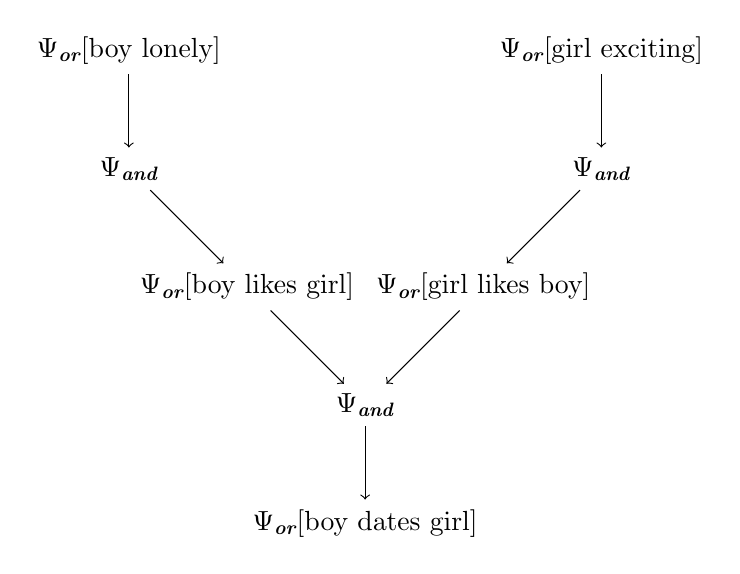
\begin{tikzpicture}
    \def\levelOne{2}
    \def\levelTwo{0.5}
    \def\levelThree{-1}
    \def\levelFour{-2.5}
    \def\levelFive{-4}
    \node (lonely) at (0,\levelOne) {$\Psi_\opor$[boy lonely]};
    \node (exciting) at (6,\levelOne) {$\Psi_\opor$[girl exciting]};
    \node (interLonely) at (0,\levelTwo) {$\Psi_\opand$};
    \node (interExciting) at (6,\levelTwo) {$\Psi_\opand$};
    \node (boyLikesGirl) at (1.5,\levelThree) {$\Psi_\opor$[boy likes girl]};
    \node (girlLikesBoy) at (4.5,\levelThree) {$\Psi_\opor$[girl likes boy]};
    \node (conjunction) at (3,\levelFour) {$\Psi_\opand$};
    \node (dates) at (3,\levelFive) {$\Psi_\opor$[boy dates girl]};
    \draw[->] (lonely) -- (interLonely);
    \draw[->] (exciting) -- (interExciting);
    \draw[->] (interLonely) -- (boyLikesGirl);
    \draw[->] (interExciting) -- (girlLikesBoy);
    \draw[->] (boyLikesGirl) -- (conjunction);
    \draw[->] (girlLikesBoy) -- (conjunction);
    \draw[->] (conjunction) -- (dates);
\end{tikzpicture}
  \caption{A {\em boolean network} that {\em alternates} between \opand\ and \opor\ gates.}
  \label{fig:alternating_network}
\end{figure}

 
\paragraph{Bipartite Graph}
Because the factor types $\Psi_\opand$ and $\Psi_\opor$ always alternate, we have a {\em bipartite graph}.
Suppose $\pvariable_1, ..., \pvariable_n$ are each {\em propositions}.
Then we say 
\begin{equation} \gvariable = \left\{\pvariable_1 \wedge ... \wedge \pvariable_n\right\} \end{equation}
is a {\em proposition group}, which are interpreted as {\em conjoined}.
Then, the two types of variables in the graph then are:
\begin{enumerate}
    \item $\pvariable$, which represents a {\em single proposition}
    \item $\gvariable$, which represents a {\em conjoined proposition group}
\end{enumerate}
For many purposes in the graphical model (e.g., {\em message passing} calculuations), we can abstract over whether a node is $\gvariable$ and $\pvariable$, and we refer to {\em generic graphical nodes} as $\zvariable$.
It is to be understood that each $\zvariable$ actually {\em wraps} a $\gvariable$ or a $\pvariable$, and that we can get either the underlying type or underlying value from any $\zvariable$ at any time.

\paragraph{Conjunction Nodes}
The {\em conjunctive} factor $\Psi_\opand$ is defined in terms of the {\em \opand\ gate}:
\begin{equation} \opand(\pvariable_1, ..., \pvariable_n) = \pvariable_1 \wedge ... \wedge \pvariable_n \end{equation}
Then:
\begin{equation}
    \Psi_{\opand}(\gvariable \condsep \pvariable_1, \ldots, \pvariable_n) = 
    \begin{cases} 
        1 & \text{if } \gvariable == \opand(\pvariable_1, \ldots, \pvariable_n), \\
        0 & \text{otherwise}
    \end{cases}
\end{equation}
It must be stressed that in all cases the $\Psi_\opand$ factor is {\em deterministic}, i.e., we do not train this even when we are interested in statistical inference.
This is owing to the fact that \opand's role is to create {\em higher-level features}, between which we can learn relationships.

\paragraph{Disjunction Nodes}
The deterministic {\em disjunctive} factor $\Psi_{\opor}$ used for the {\em completeness proof} \cite{Coppola2024}, is defined in terms of the {\em \opor\ gate}:
\begin{equation} 
    \opor(\pvariable_1, \ldots, \pvariable_n) = \pvariable_1 \vee \ldots \vee \pvariable_n 
\end{equation}
The {\em deterministic} version of \opor, used in the {\em completeness} proof, and can be used any time we want exact logical \opor, is defined as:
\begin{equation}
    \Psi_{\opor}(\gvariable \condsep \pvariable_1, \ldots, \pvariable_n) = 
    \begin{cases} 
        1 & \text{if } \gvariable == \opor(\pvariable_1, \ldots, \pvariable_n), \\
        0 & \text{otherwise}
    \end{cases}
\end{equation}
When interested in {\em statistical inference}, we {\em learn} this model, as discussed in Section \ref{sec:learned_model}.

\subsection{Markov Assumption}
The essential feature of a graphical model is that it makes a {\em Markov assumption}, in which each variable in the graph is independent of all nodes, given the values of its {\em neighbors}.
Because the edges are {\em directed}, the {\em neighbors} of a node are its {\em parents} and its {\em childen}.
In our Bayesian Network, each factor in the graph has the form:
\begin{equation} \Psi(\zvariable \condsep \zvariable_{a_1}, ..., \zvariable_{a_n}) \end{equation}
In this case, we would say that $\zvariable$ is the {\em child} of each $\zvariable_{a_i}$ and each $\zvariable_{a_i}$ is a {\em parent} of $\zvariable$.
Conversely, $\zvariable$ can also have effects on {\em its} children as in:
\begin{equation} \Psi(\zvariable_c \condsep \zvariable, \zvariable_{b_1}, ..., \zvariable_{b_{n-1}}) \end{equation}
Here, the $\zvariable_{b_i}$ are other parents of $\zvariable_c$.
The {\em Markov} assumption says that we can know everything we need to know about $\zvariable$ if we know the values of its {\em parents} and its {\em children}, i.e., $\zvariable$ is {\em independent} of all other nodes in the network, given its neighbors.

\subsection{Learned Disjunctive Model}
\label{sec:learned_model}
For the {\em learned model}, $\Psi_\opor$ is {\em learned} from {\em data}.

\paragraph{Linear Exponential Model}
For $\Psi_\opor$ we train a {\em linear exponential} model.
For a boolean variable \( \pvariable \) with boolean features \( \gvariable_1, ..., \gvariable_n \), the {\em factor potential} has the form:
\begin{equation} 
\Psi_{\opor} (\pvariable \condsep \gvariable_1, ..., \gvariable_n) = \exp{ \left\{\sum_{i=1}^{n} {\wvariable \cdot \phi(\pvariable, \gvariable_i)}\right\}}
\label{e_linear_exponential}
\end{equation}
Here, \( \wvariable \) is a weight vector, and \( \phi(\pvariable, \gvariable_i) \) is a feature discussed in Section \ref{s:feature_function}.
The probability \( P(\pvariable \condsep \gvariable_1, ..., \gvariable_n) \) is obtained by normalization over the two possible values for \( \pvariable \in \left\{0, 1\right\} \):
\begin{equation} 
P(\pvariable = p \condsep \gvariable_1, ..., \gvariable_n) = \frac{\Psi_{\opor} (p \condsep \gvariable_1, ..., \gvariable_n)}{\Psi_{\opor} (1 \condsep \gvariable_1, ..., \gvariable_n) + \Psi_{\opor} (0 \condsep \gvariable_1, ..., \gvariable_n)} 
\end{equation}

\paragraph{On the Use of a Linear Model}
One might ask whether it is {\em simplistic} to use a {\em linear} model for any reason when we have availble advanced networks like {\em multi-layer networks} and {\em attention}, etc.
The use of non-linear networks in this context can be investigated.
However, it is the role of the {\em conjunction} gates to create the {\em higher-level} features that are accomplished currently with {\em multi-layer networks}.
Linear weights are easily {\em interpretable}, which is good for {\em human-computer alignment}.
Also, for certain definitions of $\Psi_\opor$, like the {\em Noisy Or} gate discussed in Section \ref{sec:noisy_or}, updates can be {\em fast}, i.e. $O(n)$ instead of $O(2^n)$, because of the independence of inputs.
We leave it to future work to decide whether any $O(n)$ models for $\Psi_\opor$ are useful in practice.
\section{The Implication Graph}
\label{s:predgraph}
\subsection{Infinite Use of Finite Means}
Chomsky was famously fond of quoting Humboldt's aphorism that language makes {\em infinite use of finite means} \cite{Chomsky1965Aspects}.
The {\em implication graph} allows us to estimate probabilities for an {\em unbounded} number of {\em propositions} $\pvariable$ based on finite parameters $\Psi$, by defining weights over {\em predicate patterns}, rather than relationships between {\em concrete entities}.
That is, we learn a general link between $\xjack$ {\em liking} $\xjill$ and $\xjack$ {\em dating} $\xjill$, and this can apply to $\cvariable_{jack1}$ or $\cvariable_{jack2}$ or $\cvariable_{jill1}$ or $\cvariable_{jill2}$, etc., and so make {\em infinite use} of {\em finite means}.

\subsection{Graph Operations}
\paragraph{Construction}
The {\em implication graph} is constructed from the set of all relevant {\em conjoined predicate implications} that we want to train weights for in our model:
\begin{equation}
    \mathcal{K} = \left\{\Psi(\hvariable, \qvariable)\right\}
\end{equation}

\paragraph{Backwards Links for a Predicate}
From this, we can recover the {\em backwards} set of all {\em predicate implication links} for a predicate $\qvariable$:
\begin{equation}
    B_\Psi(\qvariable) = \left\{\Psi(\hvariable, \qvariable') \in \mathcal{K}  \condsep \qvariable' = \qvariable \right\}
\end{equation}
It is also possible to define a {\em forwards} set but we do not need to here.

\subsection{Abstraction and Backwards Substitution}
\paragraph{Abstraction}
For any {\em proposition} \pvariable, whose role set is $\rvariable$, we can {\em abstract} any subset of the roles in $\rvariable$ to reveal a predicate $\qvariable$.
For example, for the proposition:
\begin{equation} \pvariable = (\textsc{like}, \left\{\textsc{subj}: \constant{jack1}, \textsc{dobj}: \constant{jill1} \right\})\end{equation}
Abstracting $\left\{\textsc{subj}, \textsc{dobj}\right\}$ would leave:
\begin{equation}
    \qvariable = (\textsc{like}, \left\{\textsc{subj}: \xjack, \textsc{dobj}: \xjill \right\})
    \label{eq:}
\end{equation}
Though {\em abstracting} over all variables at once can be considered the {\em standard abstraction}, we can abstract partially
in $2^n - 1$ different ways, as $\pvariable$ is not included as an {\em abstraction} of itself, because it has no open roles.
We will write that $\qvariable \in \pvariable$ if $\qvariable$ is an abstraction of $\pvariable$.

\paragraph{Backwards Substitution}
Suppose that $\qvariable$ is an abstraction of $\pvariable$, i.e. $\qvariable \in \pvariable$.
And, suppose that $\Psi(\hvariable, \qvariable)$ is an implication link.
We can define:
\begin{equation}
    backfill(\pvariable, \Psi(\hvariable, \qvariable)) = \text{unique }\gvariable\text{ such that }\Psi(\hvariable, \qvariable)\text{ links $\gvariable$ to } \pvariable
\end{equation}
This function can be computed because we stored the {\em role mapping pair} for each $\qvariable_a \in \hvariable$ and $\qvariable$, for each $\Psi(\hvariable, \qvariable)$ in the implication graph.

\subsection{Proposition Factors and Contexts}
\paragraph{Proposition Factor}
Suppose we have a proposition $\pvariable$, which contains the predicate $\qvariable$, which matches an implication link $\Psi(\hvariable, \qvariable)$.
We can call 
$backfill(\pvariable, \Psi(\hvariable, \qvariable))$ to obtain some $\gvariable$, an instance of $\hvariable$, obtained by following backwards an instance of the link $\Psi(\hvariable, \qvariable)$.
$\gvariable = \pvariable_1 \land ... \land \pvariable_n$ is a conjunction of propositions, and so has a {\em probability}, unlike $\hvariable$, which is a predicate. These objects are all bundled up in a {\em factor} defined as:
\begin{equation}
    factor(\pvariable, \Psi(\hvariable, \qvariable)) = (\pvariable, \Psi(\hvariable, \qvariable), \gvariable)
\end{equation}
The {\em factor} contains both the causally related proposition group $\gvariable$, and also the {\em implication link} $\Psi(\hvariable, \qvariable)$ used to link $\gvariable$ and $\pvariable$.

\paragraph{Proposition Factor Context}
For a given proposition $\pvariable$, its {\em factor context} is:
\begin{equation}
    \textsc{context}(\pvariable) =
        \bigcup_{\substack{\qvariable \in \pvariable}}\ 
            \bigcup_{\substack{\hvariable \in \backlinks (\qvariable)}}
            factor(\pvariable, \Psi(\hvariable, \qvariable))
\end{equation}
This is the set of all {\em factors} created from taking all {\em backwards implication links} from all {\em abstracted predicates} $\qvariable \in \pvariable$.
The factor context is the input to the learned {\em linear exponential} model used to score the \opor\ gates, $\Psi_\opor$.
\paragraph{Markov Assumption}
In terms of the {\em Markov assumption}, the node $\pvariable$ is independent of all its ancestors given its {\em factor context}.
That is, the {\em factor context} contains the set of all {\em direct causes} for $\pvariable$, according to the current {\em theory}.

\subsection{Inference-Time Proposition Graph Creation}
When we are interested in a query $\pvariable$, we have to construct the graph of relevant proprositions {\em on the fly} at inference time, because we cannot store all propositions.
Suppose we are interested in a certain target query $\pvariable$, which for simplicity for now assume has only ancestors, and no descendents in the graph.
We can determine $context(\pvariable)$, which will get all of the conjoined nodes $\gvariable$ that are {\em parents} of $\pvariable$.
Each $\gvariable_z = \pvariable_{z_1} \wedge ... \wedge \pvariable_{z_n}$ is a conjunction of $\pvariable_{z_i}$, and for each of these we can recursively call $factor(\pvariable_{z_i})$, and so on, until we have created a {\em proposition graph} of all propositions {\em relevant to} $\pvariable$.
Because of the {\em Markov assumption}, any node not reached through this traversal is not relevant to $\pvariable$.
During the construction of this graph, we can do book-keeping to store, for each $\pvariable$ and $\gvariable$ discovered, the {\em forward} and {\em backward} links for each node of each type.

\subsection{Feature Function}
\label{s:feature_function}
The feature function $\phi(\pvariable, \gvariable)$ characterizes the {\em implication link} between the conclusion $\pvariable$ and the assumption $\gvariable$:
\begin{equation}
    \phi(\pvariable = p, \gvariable = g) = (p, \Psi(\hvariable, \qvariable), g) 
\end{equation}
That is, the feature $\phi(\pvariable = p, \gvariable = g)$ is a {\em triple} indicating:
\begin{enumerate}
    \item The value $p \in \left\{0, 1\right\}$ that $\pvariable$ takes in $\phi(\pvariable = p, \gvariable = g)$.
    \item The implication link $\Psi(\hvariable, \qvariable)$ used to arrive at $\pvariable$ from $\gvariable$.
    \item The value $g \in \left\{0, 1\right\}$ that $\gvariable$ takes on in $\phi(\pvariable = p, \gvariable = g)$.
\end{enumerate}
We usually just write $\phi(\pvariable, \gvariable)$, and assume that the $\Psi(\hvariable, \qvariable)$ is implied.
It {\em is} possible for the same $\pvariable$ and $\gvariable$ to have more than one link, which would result in more than one feature.
The {\em feature vector} for the entire {\em factor context} is the union over each of the individual {\em proposition factors}.
\section{Inference}
\label{sec:inference}
\subsection{The Probability Query}
We are interested in the \textit{probability query}, which consists of two parts:
\begin{itemize}
    \item The {\em query variables}: a subset \( \pvariableset_Q \) of all variables in the network.
    \item The {\em evidence}: a subset \( \pvariableset_E \) of random variables in the network, {\em observed} to have the values \( \left\{p\right\}_E\).
\end{itemize}
The task is to compute the {\em posterior distribution}:
\begin{equation}
    P( \pvariableset_Q \mid \pvariableset_E = \left\{p\right\}_E)
\end{equation}

\subsection{Marginalization}
In the presence of unobserved variables \( \pvariableset_U \), not part of the query or evidence, marginalization is used to sum out these variables from the joint probability distribution. The marginalization process is represented by the following equation:
\begin{equation}
    P(\pvariableset_Q \mid \pvariableset_E) = \sum_{\pvariableset_U} P(\pvariableset_Q, \pvariableset_U \mid \pvariableset_E)
\end{equation}
In general, in a Bayesian Network, this process if $\Omega(2^N)$ to compute {\em exactly}, or even to {\em provably approximate} \cite{Cooper1990,Roth1996HardnessApproxReasoning}.

\subsection{Iterative Belief Propagation}
Inference can be performed in a graphical model using {\em belief propagation} \cite{koller2009probabilistic,neapolitan2003learning,bishop2006pattern}, if the graph contains even {\em undirected cycles}, which it often would, {\em exact} belief propagation is not tractable.
However, empirical results suggest that {\em loopy belief propagation}, which we will call {\em iterative belief propagation}, does converge well empirically, even though there are no theoretical guarantees \cite{Murphy2013, Smith2008}.
We discuss the complexity of this operation in detail in Section \ref{sec:complexity}.

\subsection{Message Passing Calculations}
\paragraph{Notation}
We implement the variant of \cite{pearl1988probabilistic}'s {\em belief propagation} algorithm presented in \cite{neapolitan2003learning}.
In this formulation, we have $\pi$ {\em values} and $\lambda$ {\em values}, and $\pi$ {\em messages} and $\lambda$ {\em messages}.
For factor computations, we distinguished between {\em single propositions} $\pvariable$ and {\em proposition groups} $\gvariable$.
However, for the message passing calculations we adopt a unified notation, where both $\pvariable$ and $\gvariable$ nodes can be viewed as a unified node $\zvariable$ that can wrap either type, and the message passing calculations are agnostic to the type.
We use $\cvariable$ to canonically refer to a {\em child} of $\zvariable$ and $\avariable$ for a {\em parent} of $\zvariable$.
\paragraph{Computations}
The version we present here involves exponential cost $O(2^n)$ sums over either the parents or children of $z$.
In Section \ref{sec:complexity}, we discuss how the {\em independence} of $\Psi_\opor$ factors can, for some distributions like {\em Noisy Or}, allow the $O(2^n)$ update to be done in {\em linear} $O(n)$ time. 
\paragraph{Values}
$\pi(z)\in \mathbb{R}$, called the $\pi$ {\em value} for $\zvariable = z$, represents beliefs flowing {\em forward} in the network, from {\em causes} to {\em effects}, and is:
\begin{equation}
    \pi(z) = \sum_{a_1, \ldots, a_n} \left( P(z \mid a_1, \ldots, a_n) \prod_{a_i} \pi_\zvariable(a_i) \right).
    \label{eq:slow_pi_calc}
\end{equation}
$\lambda(z)\in \mathbb{R}$, called the $\lambda$ {\em value} for $\zvariable = z$, represents beliefs flowing {\em backward} in the network, from {\em effects} to {\em causes}, and is:
\begin{equation}
    \lambda(z) = \prod_{\cvariable} \lambda_{\cvariable}(z)
\end{equation}
These two values are normalized and combined to compute the {\em posterior} probability:
\begin{equation}P(z \condsep \left\{p\right\}_E) = \alpha\lambda(z)\pi(z) \end{equation}

\paragraph{Messages}
$\pi_\zvariable(a) \in \mathbb{R}$ is $\avariable$'s message to a {\em child} $\zvariable$:
\begin{equation}
    \pi_\zvariable(a) = \pi(a) \prod_{(\yvariable \in \zvariable) - \avariable} \lambda_\yvariable(z)
\end{equation}
$\lambda_\cvariable(z) \in \mathbb{R}$ is $\cvariable$'s message to a {\em parent} $\zvariable$, where the ${\bf b}_i$ are the other parents of $\cvariable$:
\begin{equation}
    \lambda_\cvariable(z) = \sum_{c} \left[ \sum_{b_1, b_2, \ldots, b_n} \left( P(c \mid z, b_1, b_2, \ldots, b_n) \prod_{b_i} \pi_\cvariable(b_i) \right) \lambda(c) \right]
    \label{eq_slow_lambda_calc}
\end{equation}

\section{Complexity of Inference}
\label{sec:complexity}
\subsection{Provably Exact Inference}
Inference in a general Bayesian Network is $\Omega(2^N)$ for $N$ variables, and is even $\Omega(2^N)$ to {\em provably} approximate \cite{Cooper1990, Roth1996HardnessApproxReasoning}.
\subsection{Empirically Successful Iterative Belief Propagation}
The {\em iterative belief propagation} ({\em loopy belief propagation} in the literature) is {\em not} guaranteed to converge \cite{neapolitan2003learning, koller2009probabilistic}, but {\em has been found} to converge in practice in a range of studies \cite{Smith2008, Murphy2013, Gormley2015}.
And, we have found it to converge in our experiments, which so far are small, but exhibit a recursive structure, and so thus may scale.
The primary cost of {\em inference} in this case is the computation of the {\em messages and values} of the $\pi$ and $\lambda$ tables (see Section \ref{sec:inference})
Using a perhaps {\em naive} implementation, in which the marginalization is exact (see \ref{eq:slow_pi_calc} and \ref{eq_slow_lambda_calc}), runs in time $O(2^n)$ in $n$ the number of {\em inputs} to the {\em factor}.
Then, a single pass of belief propagation visits each of the $N$ nodes once, taking total time $O(N2^n)$, and empirically $k$ rounds are needed to converge.
We remark that it may be possible to make both $\Psi_\opand$ and $\Psi_\opor$ gates faster $O(n)$, but future work must investigate.
\subsection{Faster Disjunction}
\label{sec:noisy_or}
\paragraph{Overview}
The $\Psi_\opor$ factor is {\em learned} when we want to do statistical inference, and the factor
\[\Psi_\opor(\pvariable \condsep \gvariable_1, ..., \gvariable_n)\]
has one input $n$ per {\em modeled cause} $\gvariable_i$ of $\pvariable$.
Conceptually, outcomes have an unbounded number of potential causes, and we would ideally not need to restrict $n$ solely because of message passing complexity.
\paragraph{Importance Sampling}
One option is to {\em learn} an unbounded number $n$ of weights, but only {\em consider at inference} a {\em subset} of the inputs that are most {\em relevant}.
That is, in the {\em linear exponential} model \ref{e_linear_exponential}, we can detect which of $m < n$ linear contributions will have the biggest effect, and only marginalize over those, costing $O(2^m) < O(2^n)$.
This strategy would be a variant of {\em importance sampling} \cite{wilkinson2005grammar}.
\paragraph{Linear Time Disjunction}
\cite{neapolitan2003learning} lists at least one disjunction model, the {\em Noisy Or} model, whose message passing calculations are $O(n)$, instead of $O(2^n)$ in $n$ the number of inputs to the factor.
We leave it to future work to determine whether this model, or another model with similar scaling properties, can be useful in practice.

\subsection{Faster Conjunction}
The complexity of {\em message updates} in a {\em conjunction} $\Psi_\opand$ gate is $O(2^n)$ in the number of inputs $n$.
However, an \opand\ gate can be arranged into a {\em binary tree} of \opand\ gates each of size $2$, with the tree height $\log_2(n)$, in which case there would be only $O(n)$ work in total to evaluate the $n$ inputs.
However, this would increase the amount of message passing, so we leave it to future work to evaluate whether this is beneficial.
\section{Future Work}
\paragraph{Learning from Unlabeled Text}
We have said that the {\em QBBN} can encode knowledge, and do so {\em without hallucinating}, which compares favorably with the {\em LLM} \cite{Bahdanau2014NeuralMT, vaswani2017attention, radford2018improving}.
However, the difficulty compared to the {\em LLM} is that the {\em QBBN} {\em cannot} be learned in the same {\em direct} {\em $n$-gram language model} way as the {\em LLM}, but instead must refer to {\em logical forms} which are {\em not observed} but viewed as {\em latent} and must be learned through {\em expectation maximization} \cite{dempster1977maximum}.
\paragraph{Belief Propagation}
We have used {\em loopy belief propagation}, calling it {\em iterative belief propagation}, which is not guaranteed to converge but has been studied somewhat extensively \cite{Murphy2013, Smith2008, Gormley2015}, and our experiments also find convergence.
However, convergence for larger graphs should be studied, as well as strategies to speed up belief propagation.
\paragraph{Logical Language Features}
We have shown enough about the underlying logical language of the {\em QBBN} to encode {\em basic} first-order sentences.
But, there remain the topics of {\em compositional semantics} \cite{montague1970universal}, which shows how the meanings of {\em larger parts} are made from {\em smaller parts}, and {\em intensional} semantics \cite{montague1973proper}, which shows how {\em the concept} behind a sentence can itself be an argument.
% bibliography
% \bibliographystyle{apalike}
% \bibliography{bibtex}
\begin{thebibliography}{}

    \bibitem[Bahdanau et~al., 2014]{Bahdanau2014NeuralMT}
    Bahdanau, D., Cho, K., and Bengio, Y. (2014).
    \newblock Neural machine translation by jointly learning to align and
      translate.
    \newblock {\em CoRR}, abs/1409.0473.
    
    \bibitem[Bar-Hillel, 1953]{BarHillel1953}
    Bar-Hillel, Y. (1953).
    \newblock A quasi-arithmetical notation for syntactic description.
    \newblock {\em Language}, 29(1):47--58.
    
    \bibitem[Bishop, 2006]{bishop2006pattern}
    Bishop, C.~M. (2006).
    \newblock {\em Pattern Recognition and Machine Learning}.
    \newblock Springer.
    
    \bibitem[Chomsky, 1965]{Chomsky1965Aspects}
    Chomsky, N. (1965).
    \newblock {\em Aspects of the Theory of Syntax}.
    \newblock MIT Press, Cambridge, MA.
    \newblock Available online: \url{https://mitpress.mit.edu}.
    
    \bibitem[Cooper, 1990]{Cooper1990}
    Cooper, G.~F. (1990).
    \newblock The computational complexity of probabilistic inference using
      bayesian belief networks.
    \newblock {\em Artificial Intelligence}, 42(2-3):393--405.
    
    \bibitem[Coppola, 2024]{Coppola2024}
    Coppola, G. (2024).
    \newblock A mathematical explanation for ``{Thinking Fast and Slow}''.
    \newblock Bitcoin Ordinal NFT.
    \newblock 72494446539c7fcb73becde763fc4bbbf0686b9c30cd8188e50861ccde0a5c83i0.
    
    \bibitem[Dempster et~al., 1977]{dempster1977maximum}
    Dempster, A.~P., Laird, N.~M., and Rubin, D.~B. (1977).
    \newblock Maximum likelihood from incomplete data via the em algorithm.
    \newblock {\em Journal of the Royal Statistical Society: Series B
      (Methodological)}, 39(1):1--38.
    
    \bibitem[Eisner, 2000]{eisner1996bilexical}
    Eisner, J. (2000).
    \newblock Bilexical grammars and their cubic-time parsing algorithms.
    \newblock In {\em Advances in probabilistic and other parsing technologies},
      pages 29--62. Springer.
    
    \bibitem[Gentzen, 1934]{Gentzen1934}
    Gentzen, G. (1934).
    \newblock Untersuchungen {\"u}ber das logische schlie{\ss}en.
    \newblock {\em Mathematische Zeitschrift}, 39:176--210, 405--431.
    
    \bibitem[Gilks et~al., 1996]{gilks1996markov}
    Gilks, W.~R., Richardson, S., and Spiegelhalter, D.~J., editors (1996).
    \newblock {\em Markov Chain Monte Carlo in Practice}.
    \newblock Chapman and Hall/CRC.
    
    \bibitem[G{\"o}del, 1930]{Godel1930}
    G{\"o}del, K. (1930).
    \newblock On the completeness of the calculus of logic.
    \newblock {\em Monatshefte f{\"u}r Mathematik und Physik}, 37:349--360.
    
    \bibitem[Gormley et~al., 2015]{Gormley2015}
    Gormley, M.~R., Dredze, M., and Eisner, J. (2015).
    \newblock Approximation-aware dependency parsing by belief propagation.
    \newblock {\em Transactions of the Association for Computational Linguistics},
      3:489--501.
    
    \bibitem[Kahneman, 2011]{Kahneman2011ThinkingFast}
    Kahneman, D. (2011).
    \newblock {\em Thinking, Fast and Slow}.
    \newblock Farrar, Straus and Giroux, New York.
    
    \bibitem[Koller and Friedman, 2009]{koller2009probabilistic}
    Koller, D. and Friedman, N. (2009).
    \newblock {\em Probabilistic Graphical Models: Principles and Techniques}.
    \newblock MIT Press.
    
    \bibitem[LeCun, 2023]{Lecun2023}
    LeCun, Y. (2023).
    \newblock From machine learning to autonomous intelligence.
    \newblock Ludwig-Maximilians-Universität München, YouTube.
    \newblock Accessed: 2024-01-29.
    
    \bibitem[Lewis and Steedman, 2013]{Lewis2013}
    Lewis, M. and Steedman, M. (2013).
    \newblock Combined distributional and logical semantics.
    \newblock {\em Transactions of the Association for Computational Linguistics},
      1:179--192.
    
    \bibitem[McDonald et~al., 2005]{mcdonald2005non}
    McDonald, R., Pereira, F., Ribarov, K., and Haji{\v{c}}, J. (2005).
    \newblock Non-projective dependency parsing using spanning tree algorithms.
    \newblock In {\em Proceedings of the conference on Human Language Technology
      and Empirical Methods in Natural Language Processing}, pages 523--530.
    
    \bibitem[Minsky and Papert, 1969]{minsky1969perceptrons}
    Minsky, M. and Papert, S. (1969).
    \newblock {\em Perceptrons: An Introduction to Computational Geometry}.
    \newblock MIT Press.
    
    \bibitem[Montague, 1970]{montague1970universal}
    Montague, R. (1970).
    \newblock Universal grammar.
    \newblock {\em Theoria}, 36:373--398.
    \newblock Reprinted in Thomason, Richmond H. (ed.), Formal Philosophy: Selected
      Papers of Richard Montague, pp. 7--27, Yale University Press, 1974.
    
    \bibitem[Montague, 1973]{montague1973proper}
    Montague, R. (1973).
    \newblock The proper treatment of quantification in ordinary english.
    \newblock In Hintikka, J., Moravcsik, J. M.~E., and Suppes, P., editors, {\em
      Approaches to Natural Language}, pages 221--242, Dordrecht. D. Reidel.
    
    \bibitem[Murphy et~al., 1999]{murphy1999loopy}
    Murphy, K., Weiss, Y., and Jordan, M.~I. (1999).
    \newblock Loopy belief propagation for approximate inference: An empirical
      study.
    \newblock In {\em Proceedings of the Fifteenth Conference on Uncertainty in
      Artificial Intelligence (UAI1999)}, pages 467--476. AUAI.
    
    \bibitem[Murphy et~al., 2013]{Murphy2013}
    Murphy, K.~P., Weiss, Y., and Jordan, M.~I. (2013).
    \newblock Loopy belief propagation for approximate inference: An empirical
      study.
    \newblock {\em CoRR}, abs/1301.6725.
    
    \bibitem[Neapolitan, 2003]{neapolitan2003learning}
    Neapolitan, R.~E. (2003).
    \newblock {\em Learning Bayesian Networks}.
    \newblock Prentice Hall.
    
    \bibitem[Pearl, 1988]{pearl1988probabilistic}
    Pearl, J. (1988).
    \newblock {\em Probabilistic Reasoning in Intelligent Systems: Networks of
      Plausible Inference}.
    \newblock Morgan Kaufmann.
    
    \bibitem[Pelletier, 2000]{Pelletier2000}
    Pelletier, F.~J. (2000).
    \newblock A history of natural deduction and elementary logic textbooks.
    \newblock {\em Logical consequence: Rival approaches}, 1:105--138.
    
    \bibitem[Prawitz, 1965]{Prawitz1965}
    Prawitz, D. (1965).
    \newblock {\em Natural Deduction: A Proof-Theoretical Study}.
    \newblock Stockholm Studies in Philosophy 3. Almqvist \& Wiksell, Stockholm;
      Göteborg; Uppsala.
    \newblock Acta Universitatis Stockholmiensis.
    
    \bibitem[Radford et~al., 2018]{radford2018improving}
    Radford, A., Narasimhan, K., Salimans, T., and Sutskever, I. (2018).
    \newblock Improving language understanding by generative pre-training.
    
    \bibitem[Richardson and Domingos, 2006]{richardson2006markov}
    Richardson, M. and Domingos, P. (2006).
    \newblock Markov logic networks.
    \newblock {\em Machine learning}, 62:107--136.
    
    \bibitem[Roth, 1996]{Roth1996HardnessApproxReasoning}
    Roth, D. (1996).
    \newblock On the hardness of approximate reasoning.
    \newblock {\em Artificial Intelligence}, 82:273--302.
    
    \bibitem[Smith and Eisner, 2008a]{Smith2008}
    Smith, D. and Eisner, J. (2008a).
    \newblock Dependency parsing by belief propagation.
    \newblock In Lapata, M. and Ng, H.~T., editors, {\em Proceedings of the 2008
      Conference on Empirical Methods in Natural Language Processing}, pages
      145--156, Honolulu, Hawaii. Association for Computational Linguistics.
    
    \bibitem[Smith and Eisner, 2008b]{smith2008dependency}
    Smith, D.~A. and Eisner, J. (2008b).
    \newblock Dependency parsing by belief propagation.
    \newblock In {\em Proceedings of the 2008 Conference on Empirical Methods in
      Natural Language Processing}, pages 145--156.
    
    \bibitem[Steedman, 1996]{Steedman1996}
    Steedman, M. (1996).
    \newblock {\em Surface Structure and Interpretation}.
    \newblock The MIT Press.
    
    \bibitem[Sutskever, 2023]{SutskeverObservation}
    Sutskever, I. (2023).
    \newblock An observation on generalization.
    \newblock Simons Institute, YouTube.
    \newblock Accessed: 2024-01-29.
    
    \bibitem[Vaswani et~al., 2017a]{vaswani2017attention}
    Vaswani, A., Shazeer, N., Parmar, N., Uszkoreit, J., Jones, L., Gomez, A.~N.,
      Kaiser, L., and Polosukhin, I. (2017a).
    \newblock Attention is all you need.
    \newblock In {\em Advances in Neural Information Processing Systems},
      volume~30.
    
    \bibitem[Vaswani et~al., 2017b]{Vaswani2017}
    Vaswani, A., Shazeer, N., Parmar, N., Uszkoreit, J., Jones, L., Gomez, A.~N.,
      Kaiser, L., and Polosukhin, I. (2017b).
    \newblock Attention is all you need.
    \newblock In {\em Advances in Neural Information Processing Systems},
      volume~30.
    
    \bibitem[Wilkinson, 2005]{wilkinson2005grammar}
    Wilkinson, L. (2005).
    \newblock {\em The Grammar of Graphics}.
    \newblock Springer, 2 edition.
    
    \bibitem[Zhang and Nivre, 2011]{zhang2011transition}
    Zhang, Y. and Nivre, J. (2011).
    \newblock Transition-based dependency parsing with rich non-local features.
    \newblock In {\em Proceedings of the 49th Annual Meeting of the Association for
      Computational Linguistics: Human Language Technologies}, pages 188--193.
    
    \end{thebibliography}
    
% end
\end{document}
